\documentclass[
    a4paper,     %% defines the paper size: a4paper (default), a5paper, letterpaper, ...
    % landscape,   %% sets the orientation to landscape
    % twoside,     %% changes to a two-page-layout (alternatively: oneside)
    % twocolumn,   %% changes to a two-column-layout
        headsepline, %% add a horizontal line below the column title
    % footsepline, %% add a horizontal line above the page footer
    % titlepage,   %% only the titlepage (using titlepage-environment) appears on the first page (alternatively: notitlepage)
        halfparskip,     %% insert an empty line between two paragraphs (alternatively: halfparskip, ...)
    % leqno,       %% equation numbers left (instead of right)
        fleqn,       %% equation left-justified (instead of centered)
    % tablecaptionabove, %% captions of tables are above the tables (alternatively: tablecaptionbelow)
    % draft,       %% produce only a draft version (mark lines that need manual edition and don't show graphics)
    % 10pt         %% set default font size to 10 point
    % 11pt         %% set default font size to 11 point
    10pt         %% set default font size to 12 point
    ]{scrartcl}  %% article, see KOMA documentation (scrguide.dvi)
    
    
    
%%%%%%%%%%%%%%%%%%%%%%%%%%%%%%%%%%%%%%%%%%%%%%%%%%%%%%%%%%%%%%%%%%%%%%%%%%%%%%%%
%%%
%%% packages
%%%
        
%%%
%%% encoding and language set
%%%

\usepackage[english]{babel}

%%% inputenc: coding of german special characters
\usepackage[latin1]{inputenc}

%%% fontenc, ae, aecompl: coding of characters in PDF documents
\usepackage[T1]{fontenc}
\usepackage{ae,aecompl}

\usepackage{xcolor}

%%%
%%% technical packages
%%%

\usepackage{listings}
\definecolor{green_code}{rgb}{0,0.6,0}
\lstdefinestyle{myCodeSnippetStyle}{
    language = python,
    commentstyle = \color{green_code},
    basicstyle = \footnotesize,
    gobble = 8,
    frame = single
}
\lstset{style = myCodeSnippetStyle}

\usepackage{tikz}
\usetikzlibrary{patterns}

\usepackage{pgfplots}
\pgfplotsset{compat = 1.16}

\usepackage{multirow}

%%% amsmath, amssymb, amstext: support for mathematics
\usepackage{amsmath,amssymb,amstext, amsthm}
        
%%%%%%%%%%%%%%%%%%%%%%%%%%%%%%%%%%%%%%%%%%%%%%%%%%%%%%%%%%%%%%%%%%%%%%%%%%%%%%%%
%%%
%%% user defined commands
%%%

\newtheorem{lemma}{Lemma}[section]

\newtheorem{theorem}{Theorem}[section]

\newtheorem{corollary}{Corollary}[section]

\newtheorem{proposition}{Proposition}[section]

\theoremstyle{definition}
\newtheorem{definition}{Definition}[section]

\theoremstyle{remark}
\newtheorem*{remark}{Remark}

\theoremstyle{remark}
\newtheorem{example}{Example}
        
\newcommand{\nats}{\mathbb{N}}
\newcommand{\reals}{\mathbb{R}}

\newcommand{\argmin}{\operatorname{argmin}}
\newcommand{\argmax}{\operatorname{argmax}}

%%%%%%%%%%%%%%%%%%%%%%%%%%%%%%%%%%%%%%%%%%%%%%%%%%%%%%%%%%%%%%%%%%%%%%%%%%%%%%%%
%%%
%%% define the titlepage
%%%

\subject{Modelling week 2022}   %% subject which appears above titlehead
% \titlehead{} %% special heading for the titlepage

%%% title
\title{My notes on mathematical game theory}

%%% author(s)
\author{Florian Thaler}

%%% date
\date{Graz, Sommersemester 2022}

% \publishers{}

% \thanks{} %% use it instead of footnotes (only on titlepage)

% \dedication{} %% generates a dedication-page after titlepage


%%%%%%%%%%%%%%%%%%%%%%%%%%%%%%%%%%%%%%%%%%%%%%%%%%%%%%%%%%%%%%%%%%%%%%%%%%%%%%%%
%%%
%%% begin document
%%%

\begin{document}

    \maketitle

    \tableofcontents
    \newpage
    \section{Basics}
        Mathematical game theory considers single or repeated interactions between several so called rational players. A player is said to be rational if he 
tries to maximise his own payoff. Additionally it is assumed that all the players make their decisions simultaneously and independent from each other.

\begin{definition}\label{def:game}
    Let $n\in\nats$, $\mathcal{P} = \{1, \ldots, n\}$, let $S_{1}, \ldots, S_{n}$ be non-empty sets and let $\pi_{i}:S\to\reals$, $1\leq i\leq n$, where
    $S = \prod_{i = 1}^{n}S_{i}$. Letting $\pi = (\pi_{1}, \ldots, \pi_{n})$, the pair $G = (S, \pi)$ is called a $n$ player strategic game with set
    of players $\mathcal{P}$. For every player $i\in\mathcal{P}$ the set $S_{i}$ is called the set of strategies and the mapping 
    $\pi_i$ is called the payoff function of the $i$-th player.
\end{definition}

\begin{remark}
    A strategy in this context is an action or a control which a player will take or apply.
\end{remark}

There is no general solution concept of a strategic game, and hence no general definition of what exactly a solution is in this context. There are different 
approaches like Nash equilibrium, Pareto optimality, or strict dominance with the purpose of finding strategies
which are in a certain sense optimal for the players involved. We will introduce here only the concept of Nash equilibria. Before introducing this concept some
examples are listed and discussed.

\begin{example}[The prisoner's dilemma] 
    Two suspects in a severe crime and a small robbery are put into separate cells. Both are in solitary confinemnent, which does not give them the possibility
    to communicate with each other. The police has enough evidence to convict them for the robbery, but no evidence for the more severe crime. Thus the police
    gives both of them the offer to confess: If both of them confess the crime, then both will spend 10 years in jail. If only one confesses and acts as a
    withness against the other, he will receive no punishment, where the other one will be sent to jail for 15 years. If none of them confesses both will be judged
    for the rubbery and will be sent to jail for 1 year each. The courses of action open to each prisoner is $q$ = keep quiet, or $s$ = squeal. The payoffs of each 
    player are given in terms of freedom lost. In the notation of Definition \ref{def:game} we have
    \begin{enumerate}
        \item $S_{1} = S_{2} = \{q, s\}$
        \item $\pi_{1}(q, q) = -1$, $\pi_{1}(q, s) = -15$, $\pi_{1}(s, q) = 0$, $\pi_{1}(s, s) = -10$, and 
                $\pi_{2}(q, q) = -1$, $\pi_{2}(q, s) = 0$, $\pi_{2}(s, q) = -15$, $\pi_{2}(s, s) = -10$.
    \end{enumerate}
    Hence we infer that the prisoner's dilemma is a strategic game in the sense of Definition \ref{def:game}. A convenient way to represent this game and more general
    strategic games of small strategy sets is the following 
    \newline
    \begin{center}
        \begin{tabular}{c | r | c | c |}
            \multicolumn{2}{c}{} & \multicolumn{2}{c}{Player 2}\\
            \cline{2-4}
            & & $q$ & $s$ \\
            \cline{2-4}
            \multirow{2}{*}{Player 1} & $q$ & (-1, -1) & (-15, 0) \\
            \cline{2-4}
            & $s$ & (0, -15) & (-10, -10)) \\
            \cline{2-4}
        \end{tabular}            
    \end{center}
    What should each of the prisoners do - which strategy should any of them choose? Let us consider first player 1. If player 2 keeps quiet, then player 1 should squeal
    in order to minimize the number of years he has to go to jail. If on the other hand player 2 squeals, then also player 1 should squeal. This means player 1 should - 
    following this reasoning - squeal in any case. Similarly player 2 should always squeal. But the table shows that if both of the prisoners follow their self-interests 
    (minimizing the number number years in jail) they will end up worse as if they kept quiet. This observation makes this example so interesting. The fact that
    the prisoner's dilemma has a lot of applications in real world makes it even more interesting. Consider it for example in the context of the cold war or in the context
    of paying taxes. Whatever any person does - in regard of our personal financial wealth it pays off to pay no taxes. But if no taxes are paid, then there is no money
    for common goods. Thus the community is worse off than if people would have paid their taxes.
\end{example}

\begin{example}[First price auction]
    Let us consider an auction of a single object. Let us assume that there is a set of $n$ bidders. Each of the assigns the object a value - let $v_{i}$ the value assigned
    by the $i$-th bidder. For the sake of simplicity we assume that $v_{1} > \ldots > v_{n} > 0$. The auction is held as follows:
    \begin{enumerate}
        \item The players submit their bid simultaneously and independently
        \item The object is assigned to the player with the smallest index among the players which placed the largest bid.
        \item The players which gets the object pays the bid.
    \end{enumerate}
    This auction defines a strategic $n$ player game $G = (S, \pi)$, where $S_{i} = \reals_{\geq0}$ and 
    \begin{align*}
        \pi_{k}(s_{1}, \ldots, s_{n}) = 
            \begin{cases}
                v_{i} - s_{i} \text{ if } i = \max\{k : 1\leq k\leq n, a_{k} = max_{1\leq l\leq n}s_{l}\} \\
                0 \text{ else}
            \end{cases}
    \end{align*}
    for $i = 1, \ldots, n$.
\end{example}

\begin{example}[Matching pennies]\label{ex:pennies}
    Two players place simultaneously and independently a penny on a table - or heads up (strategy $h$) or tails up (strategy $t$). If the pennies match (i.e. both heads or both
    tails) then player 1 wins and keeps both pennies. In the other case player 2 wins and gets both pennies. The game can be represented in tabular form as follows
    \newline
    \begin{center}
        \begin{tabular}{c | r | c | c |}
            \multicolumn{2}{c}{} & \multicolumn{2}{c}{Player 2}\\
            \cline{2-4}
            & & $h$ & $t$ \\
            \cline{2-4}
            \multirow{2}{*}{Player 1} & $h$ & (1, -1) & (-1, 1) \\
            \cline{2-4}
            & $t$ & (-1, 1) & (1, -1)) \\
            \cline{2-4}
        \end{tabular}            
    \end{center}
    We may pose the question:
    \begin{addmargin}[75pt]{0pt}
        Is there a strategy pair such that no player gains 
        \newline
        when unilaterally deviating from it?
    \end{addmargin}
    In the given case there is none. Let us consider exemplary the case where both of the players play head. Then for player 2 it would pay off if he would play tale.
\end{example}

Any pair of strategies having the property mentioned in Example \ref{ex:pennies} is called a Nash equilibrium, which will be introduced more formally next. For the sake of
simplicity we will consider henceforth only two player games. The principles can be generalised easily to more general situations - see \cite{webb2007game}, \cite{gonzalez2010introductory}.

\begin{definition}
    Let $G = (S, \pi)$ be a strategic game, and let $\sigma_{1}^{*}\in S_{1}$, $\sigma_{2}^{*}\in S_{2}$. Then $(s_{1}^{*}, s_{2}^{*})$ is called a
    Nash equilibrium if 
    \begin{equation*}
        \pi_{1}(s_{1}^{*}, s_{2}^{*}) \geq \pi_{1}(s_{1}, s_{2}^{*}), s_{1}\in S_{1} \text{ and }
            \pi_{2}(s_{1}^{*}, s_{2}^{*}) \geq \pi_{2}(s_{1}^{*}, s_{2}), s_{2}\in S_{2}.
    \end{equation*}
\end{definition}

\begin{remark}
    \begin{enumerate}
        \item There can be more than one Nash equilibrium, i.e. Nash equilibria are not unique.
        \item Not every game has a Nash equilibrium as Example \ref{ex:pennies} indicates. However it can be shown that strategic games under certain 
            assumptions do always have at least one Nash uquilibrium. This result is known as Nash's theorem, which will be stated down below without
            proof.
        \item The pair $(s, s)$ is a Nash equilibrium for the prisoner's dilemma. 
    \end{enumerate}
\end{remark}

Before stating Nash's theorem let us introduce some notation. For every $x\in\reals^{k}$, every $1\leq i\leq k$ and every $y\in\reals$ we write
\begin{equation*}
    x_{-i} = (x_{1}, \ldots, x_{i - 1}, x_{i + 1}, \ldots, x_{k}) ~\text{ and }~ (x_{-i}, y) = (x_{1}, \ldots, x_{i - 1}, y, x_{i + 1}, \ldots, x_{k}).
\end{equation*}
For a function $f$ defined on a subset of $\reals^{k}$ we further denote by $f(x_{-i}, \cdot)$ the mapping defined by
\begin{equation*}
    f(x_{-i}, \cdot)(y) = f(x_{-i}, y),
\end{equation*}
for suitable $x\in\reals^{k}$, $y\in\reals$.

\begin{theorem}[Nash's theorem]
    Let $G = (S, \pi)$ be a strategic game such that for every $i = 1, 2$ the following assumptions hold:
    \begin{enumerate}
        \item $S_{i}$ is a non-empty, convex and compact subset of $\reals^{k_{i}}$ for some $k_{i}\in\nats$
        \item $\pi_{i}$ is continuous
        \item For every $s\in S_{i}$ the function $\pi_{i}(s_{-i}, \cdot)$ is quasi-concave on $S_{i}$, i.e. for every $x, y \in\reals$ such that
            $(s_{-i}, x), (s_{-i}, y)\in S_{i}$ and every $t\in[0, 1]$ it holds 
            \begin{equation*}
                \pi_{i}(s_{-i}, \cdot)(tx + (1 - t)y)\geq\min(\pi_{i}(s_{-i}, \cdot)(x), \pi_{i}(s_{-i}, \cdot)(y)).
            \end{equation*}
    \end{enumerate}
    Then $G$ has at least one Nash equilibrium.
\end{theorem}

For a proof of this theorem see for example \cite{gonzalez2010introductory}, Section 2.2.

So far we considered only so called pure strategies. This refers to situation where any player plays exactly (in a deterministic manner) only the strategies which 
are available in its strategy set. We will introduce now as well so called mixed strategies in the case where the strategy set of each player is finite. Games of this
kind are called finite.

\begin{definition}
    Let $G = (S, \pi)$ be a finite strategic game and let $\mathcal{D}(S_{i})$, $i = 1, 2$ be the set of all probability distributions over the set $S_{i}$. Then any probability
    distribution $\mu_{i}\in\mathcal{D}(S_{i})$ is called a mixed strategy of the $i$-th player.
\end{definition}

\begin{remark}
    \begin{enumerate}
        \item Every pure strategy is also a mixed strategy.
        \item Each of the sets $\mathcal{D}(S_{i})$ can be identified with
            \begin{equation*}
                \Sigma_{i} = \{(\sigma_{1}, \ldots, \sigma_{m_{i}})\in\reals_{\geq0}^{m_{i}} : \sum_{j = 1}^{m_{i}}\sigma_{j} = 1\},
            \end{equation*}
            where $m_{i} = |S_{i}|$. Consequently any mixed strategy can be respresented by a probability vector $\sigma\in\reals_{\geq0}^{m_{i}}$, where
            its $j$-th component $\sigma_{j}$ corresponds to the probability with which the pure strategy $s_{j}\in S_{i}$ is chosen. To point this
            out we write also $\sigma_{j} = p^{(i)}(s_{j})$.
        \item Representing pure strategies $s_{j}\in S_{i}$ by means of the canonical basis vectors in $\reals^{m_{i}}$, $m_{i} = |S_{i}|$, i.e.
            \begin{equation*}
                s_{j} = (0, \ldots, 0, 1, 0, \ldots, 0),
            \end{equation*}
            allows to write each mixed $\sigma\in\Sigma_{i}$ as linear combination of pure strategies as follows
            \begin{equation*}
                \sigma = \sum_{j = 1}^{m_{i}}\sigma_{j}s_{j} = \sum_{j = 1}^{m_{i}}p^{(i)}(s_{j})s_{j}
            \end{equation*}
        \item To look at mixed strategies is particularly interesting in the case of repeated games. Since each strategy is probabilistic, neither player knows
            for sure which plan of action the other player will use (plan of action is not predictible). 
    \end{enumerate}
\end{remark}

\begin{definition}
    Let $G = (S, \pi)$ be a finite strategic game. Then the mixed extension of $G$ is the game $\mathcal{E}(G) = (\Sigma, \hat{\pi})$, where 
    $\Sigma = \Sigma_{1}\times\Sigma_{2}$ and 
    \begin{equation*}
         \hat{\pi}_{i}(\sigma_{1}, \sigma_{2}) 
            = \sum_{s_{1}\in S_{1}, s_{2}\in S_{2}}\pi_{i}(s_{1}, s_{2})p^{(l)}(s_{1})p^{(l)}(s_{2}), ~~ \sigma_{l} = \sum_{s\in S_{l}}p^{(l)}(s)s, ~l = 1, 2
    \end{equation*}
    for $i = 1, 2$.
\end{definition}

\begin{remark}
    \begin{enumerate}
        \item The mixed extension $\mathcal{E}(G)$ is again a strategic game in the sense of Definition \ref{def:game}
        \item Note, that $\hat{\pi}_{i}$ and $\pi_{i}$ coincide on $S$, thus $\hat{\pi}_{i}$ is an extension of $\pi$ to $\Sigma$. For the sake of readibility
            we do not distinguish between $\pi_{i}$ and $\hat{\pi}_{i}$.
        \item Let $|S_{1}| = m_{1}$, $|S_{2}| = m_{2}$. Let us identify $S_{1}$, $S_{2}$ with the sets $\{1, \ldots, m_{1}\}$
            and $\{1, \ldots, m_{2}\}$ respectively. Definining the matrices $A_{1}, A_{2}\in\reals^{m_{1}\times m_{2}}$ via
            \begin{equation*}
                A_{l} = (\pi_{l}(i, j))_{1\leq i\leq m_{1}, 1\leq j\leq m_{2}}, ~l = 1, 2
            \end{equation*}
            we can write
            \begin{align*}
                \pi_{i}(\sigma_{1}, \sigma_{2}) = \sigma_{1}A_{i}\sigma_{2}^{T}, ~ i = 1, 2.
            \end{align*}
            In this case the game can entirely be characterised by the matrices $A_{1}, A_{2}$. A game of this kind is called bimatrix game.
    \end{enumerate}
\end{remark}

\begin{corollary}
    Let $G = (S, \pi)$ be a finite strategic game. Then the mixed extension $\mathcal{E}(G)$ of $G$ has a Nash equilibrium.
\end{corollary}

\begin{example}[Matchig pennies - mixed extension]\label{ex:pennies_mixed}
    Consider the mixed strategies $\sigma_{1} = (p, 1 - p)$, $\sigma_{2} = (q, 1 - q)$ for player $1$ and player $2$. Hence player $1$ plays heads
    with probability $p$ and plays tails with probability $1 - p$ - the analogous statement holds for player $2$ with $q$ instead of $p$. 
    The payoffs are given as
    \begin{align*}
        &\pi_{1}(\sigma_{1}, \sigma_{2}) = pq - p(1 - q) - (1 - p)q + (1 - p)(1 - q) = 1 - 2q + 2p(2q - 1), \\
        &\pi_{2}(\sigma_{1}, \sigma_{2}) = -pq + p(1 - q) + (1 - p)q - (1 - p)(1 - q) = -1 + 2p - 2q(2p - 1)
    \end{align*}
    We aim to find values for $p, q \in[0, 1]$ such that a Nash equilibrium appears. Let us define $f_{1}(p, q) = 1 - 2q + 2p(2q - 1)$ and 
    $f_{2} =  -1 + 2p - 2q(2p - 1)$ on $[0, 1]^{2}$ respectively. Since
    \begin{align*}
        \partial_{1}f_{1}(p, q) = 2(2q - 1), ~~~ \partial_{2}f_{2}(p, q) = -2(2p - 1)
    \end{align*}
    we infer first $f_{1}(p, 1 / 2)\geq f_{1}(p, q)$ and $f_{2}(1 / 2, q)\geq f_{2}(p, q)$. Since $f_{1}(1 / 2, 1 / 2) = f_{1}(p, 1 / 2)$ and 
    $f_{2}(1 / 2, 1 / 2) = f_{2}(1 / 2, q)$ for every $p, q$ we conclude that the mixed strategies according to $p = 1 / 2$ and $q = 1 / 2$ 
    build a Nash equilibrium.
\end{example}

\begin{example}[Penalty kicks]\label{ex:penalties}
    Let us consider a simplified penalty kick sitation in football. We make the following simplifying assumptions
    \begin{itemize}
        \item Kicker and goalkeeper act simultaneously and independently.
        \item Kicker and goalkeeper have only two choices: kick left/right and jump left/right respectively
        \item If both choose the same side, then the goalkeeper saves the penalty.
        \item The kicker is right-footed, which makes it more likely that he scores when kicking to the left
    \end{itemize}
    The tabular form of the game is as follows
    \begin{center}
        \begin{tabular}{c | r | c | c |}
            \multicolumn{2}{c}{} & \multicolumn{2}{c}{Goalkeeper}\\
            \cline{2-4}
            & & $l$ & $r$ \\
            \cline{2-4}
            \multirow{2}{*}{Kicker} & $l$ & (0, 0) & (2, -2) \\
            \cline{2-4}
            & $r$ & (1, -1) & (0, 0)) \\
            \cline{2-4}
        \end{tabular}            
    \end{center}
    We aim to find Nash equilibria of this game. We observe that this game has no pure Nash equilibrium. Let us for example comsider the pair $(l, r)$, i.e.
    the kicker shoots left and the goalkeeper jumps to the right. Then the goalkeeper could increase his payoff if jumping to the left.
    Let us now consider the mixed strategies $\sigma_{1} = (p, 1 - p)$, $\sigma_{2} = (q, 1 - q)$. Then it holds
    \begin{align*}
        &\pi_{1}(\sigma_{1}, \sigma_{2}) = 2p (1 - q) + (1 - p) q = 2p - 3pq + q\\
        &\pi_{2}(\sigma_{1}, \sigma_{2}) = -2p (1 - q) - (1 - p) q = 3pq - 2p - q
    \end{align*}
    Using the same approach as in Example \ref{ex:pennies_mixed} we find a Nash equilibrium for $p = 1 / 3$, $q = 2 / 3$.
\end{example}

    % \begin{example}[The instigation game]
        
    % \end{example}

\begin{example}[Battle of the sexes]
    A man and a woman would like to go out for a date and decide to go to a concert. They have two choices - Metallica ($M$) or The Editors ($E$). Florian perfers 
    Metallica and Susanne prefers The Editors. Both would like to go the same event rather than to go to different concerts. We model this situation by means
    of a strategic game. The tabular form of it is given by
    \begin{center}
        \begin{tabular}{c | r | c | c |}
            \multicolumn{2}{c}{} & \multicolumn{2}{c}{Susanne}\\
            \cline{2-4}
            & & $M$ & $E$ \\
            \cline{2-4}
            \multirow{2}{*}{Florian} & $M$ & (3, 2) & (1, 1) \\
            \cline{2-4}
            & $E$ & (0, 0) & (2, 3)) \\
            \cline{2-4}
        \end{tabular}            
    \end{center}
    We infer that this game has two pure strategiy pairs forming a Nash equilibrium, namely $(M, M), (E, E)$. Additionally one can prove that this
    game has as well a Nash equilibrium consisting of mixed strategies. But how should the couple decide? In the literature several approaches to 
    deal with such situations are discussed. One could for example use a convention, or generalise the solution concept of Nash (correlated equilibrium).
\end{example}
        \newpage

    \section{Matrix games}
        In this section we discuss a special class of games - so called matrix games, which are a special case of bimatrix games. As in the first section we 
consider also here finite two player games.

\begin{definition}
    A strategic game $G = (S, \pi)$ is called a zero-sum game if $\pi_{1}(s_{1}, s_{2}) + \pi_{2}(s_{1}, s_{2}) = 0$ for every $(s_{1}, s_{2})\in S$.
\end{definition}

\begin{definition}
    Let $G = (S, \pi)$ be a zero-sum game. Then its mixed extension is called a matrix game.
\end{definition}

\begin{remark}
    Let $S_{1} = \{1, \ldots, m_{1}\}, S_{2} = \{1, \ldots, m_{2}\}$ and let $A\in\reals^{m_{1}\times m_{2}}$ defined by
    \begin{equation*}
        A = (\pi_{1}(i, j))_{1\leq i\leq m_{1}, 1\leq j\leq m_{2}}.
    \end{equation*}
    Then it holds
    \begin{equation*}
        \pi_{1}(\sigma_{1}, \sigma_{2}) = \sigma_{1}A\sigma_{2}^{T} ~~ and ~~ \pi_{1}(\sigma_{1}, \sigma_{2}) = -\sigma_{1}A\sigma_{2}^{T}
    \end{equation*}s
    for all $(\sigma_{1}, \sigma_{2})\in\Sigma$.
\end{remark}

For this special class of games we consider next to Nash equilibria another solution concept which was first introduced by John v. Neumann and is based
on the so called value of a game.

\begin{definition}
    Let $G = (S, \pi)$ be a game.
    \begin{enumerate}
        \item $v_{L} = \sup_{s_{1}\in S_{1}}\inf_{s_{2}\in S_{2}}\pi_{1}(s_{1}, s_{2})$, $v_{U} = \inf_{s_{2}\in S_{2}}\sup_{s_{1}\in S_{1}}\pi_{1}(s_{1}, s_{2})$
            are called the lower value and the upper value of $G$ respectively.
        \item If $v_{L} = v_{U}$, then the game is called strictly determined or said to have a value. In this case $v = v_{L}$ is called the value of the game.
    \end{enumerate}
\end{definition}

Let us define the mappings $\varphi:S_{1}\to\reals$, $\psi:S_{2}\to\reals$ via $\varphi(s_{1}) = \inf_{s_{2}\in S_{2}}\pi_{1}(s_{1}, s_{2})$ and 
$\psi(s_{2}) = \sup_{s_{1}\in S_{1}}\pi_{1}(s_{1}, s_{2})$. Then $\varphi(s_{1})$ refers to the worst payoff player $1$ receives if applying $s_{1}$,
and $\psi(s_{2})$ gives the maximal loss player $2$ can make when playing $s_{2}$. Thus a conservative, but suitable strategy for player $1$ may be to choose
a strategy which is maximising $\varphi$. Similarly player $2$ may seek a strategy which minimises $\psi$. 

\begin{definition}\label{def:optSol}
    Let $G = (S, \pi)$ be a game. 
    \begin{enumerate}
        \item Any $s_{1}^{*}\in S_{1}$ satisfying
            \begin{equation*}
                \varphi(s_{1}^{*}) = \sup_{s_{1}\in S_{1}}\varphi(s_{1})
            \end{equation*}
            is called a maximin strategy for player $1$.
        \item Let $s_{2}^{*}\in S_{2}$ such that
            \begin{equation*}
                \psi(s_{2}^{*}) = \inf_{s_{2}\in S_{2}}\psi(s_{2}).
            \end{equation*}
            Then $s_{2}^{*}$ is called a minimax strategy for player $2$.
    \end{enumerate}
\end{definition}

In general we cannot assume that a maximin strategy for player $1$ or a minimax strategy for player $2$ exists. Let us consider now the special case of a
matrix game. Let $A\in\reals^{m_{1}\times m_{2}}$ be the matrix corresponding to the payoff function $\pi{1}$. Due to compactness of $\Sigma_{1}$, 
$\Sigma_{2}$ and the continuity of bilinear functions we have
\begin{equation*}
    \varphi(\sigma_{1}) = \min_{\sigma_{2}\in\Sigma_{2}}\sigma_{1}A\sigma_{2}^{T} ~\text{ and }~ \psi(\sigma_{1}) = \max_{\sigma_{1}\in\Sigma_{1}}\sigma_{1}A\sigma_{2}^{T}
\end{equation*}

As the following Lemma states, the minimum in the definition of $\varphi$ and the maximum in the definition of $\psi$ is attained among the set of pure strategies.

\begin{lemma}
    For every $\sigma_{1}\in\Sigma_{1}$ and every $\sigma_{2}\in\Sigma_{2}$ it holds
    \begin{equation*}
        \varphi(\sigma_{1}) = \min_{1\leq j\leq m_{2}}\sigma_{1} Ae_{j}^{T} ~\text{ and }~ \psi(\sigma_{2}) = \max_{1\leq i\leq m_{1}}e_{i} A\sigma_{2}^{T}
    \end{equation*}
\end{lemma}
\begin{proof}
    Shouldn't be hard.
\end{proof}

According to the above statement we have in particular the following relations for the upper and lower value of the game
\begin{equation*}
    v_{L} = \max_{\sigma_{1}\in\Sigma_{1}}\min_{1\leq j\leq m_{2}}\sigma_{1} Ae_{j}^{T}, ~~ 
        v_{U} = \min_{\sigma_{2}\in\Sigma_{2}}\max_{1\leq i\leq m_{1}}e_{i} A\sigma_{2}^{T}.
\end{equation*}
Obviously it holds $v_{L}\leq v_{U}$, but it is not that obvious that also the reverse inequality holds true. This is the statement of the next theorem.

\begin{theorem}[Minimax theorem]
    Every matrix game is strictly determined.
\end{theorem}

For a proof of this theorem see for example section 2.6 in \cite{gonzalez2010introductory}. As a consequence we have that strategies $\sigma_{1}^{*}\in\Sigma_{1}$,
$\sigma_{2}^{*}\in\Sigma_{2}$ are optimal for player $1$ and player $2$ respectively in the sense of Definition \ref{def:optSol}, if 
\begin{equation*}
    \varphi(\sigma_{1}^{*}) = v = \psi(\sigma_{2}^{*}).
\end{equation*}

As the following results address, the solution concepts we were discussing, i.e. the concept of Nash equilibria and the concept of maximin and minimax solutions correlate.

\begin{proposition}
    Let $G = (S, \pi)$ be a zero-sum game, and let $(s_{1}^{*}, s_{2}^{*})\in S$ be a Nash equilibrium. Then the following statements hold true:
    \begin{enumerate}
        \item G is strictly determined 
        \item $s_{1}^{*}$ is a maximin strategy for player $1$ and $s_{2}^{*}$ is a minimax strategy for player $2$
        \item $v = u_{1}(s_{1}^{*}, s_{2}^{*})$
    \end{enumerate}
\end{proposition}

\begin{proposition}\label{prop:minimaxNash}
    Let $G = (S, \pi)$ be a zero-sum game. Let $G$ be strictly determined and let $(s_{1}^{*}$, $s_{2}^{*})\in S$ be a maximin and minimax strategy 
    for player $1$ and player $2$ respectively. Then $(s_{1}^{*}, s_{2}^{*})$ is a Nash equilibrium of $G$ and it holds $v = u_{1}(s_{1}^{*}, s_{2}^{*})$.
\end{proposition}

For the proofs of both of the statements see section 2.3 in \cite{gonzalez2010introductory}.

For matrix games it turns out that the maximin and the minimax strategies for player $1$ and player $2$ respectively can be found numerically in a 
rather convenient way\footnote{The approach presented here follows mainly \cite{lavrov}, \cite{mansour}}. Let us have again have a look on how these
 strategies are defined. The maximin strategy for player $1$ is by definition the solution of the optimisation problem
\begin{align*}
    \begin{cases}
        \max_{x\in\reals^{m_{1}}}\min_{1\leq j\leq m_{2}}xAe_{j}^{T} ~\text{ subject to}\\   
        ~~~~ x_{1} + \ldots + x_{m_{1}} = 1\\
        ~~~~ x_{1}, \ldots, x_{m_{1}}\geq 0
    \end{cases}
\end{align*}
Using a simple trick this optimisation problem can be transformed into a linear program. We note that the minimum of several terms can be 
maximised, by maximising an auxiliary variable $z$ subject to the constraint that $z$ is less or equal than every term of which the minimum is taken.
Using this approach and letting denote $\mathbf{0}, \mathbf{1}\in\reals^{m_{1}}$ the vectors whos components are equal $0$ and $1$ respectively, the
problem we aim to solve reads
\begin{align*}
    (LP_{1})
    \begin{cases}
        \max_{x\in\reals^{m_{1}}, z\in\reals}z ~\text{ subject to}\\   
        ~~~~  - xA \leq -z\mathbf{1}\\
        ~~~~ x\mathbf{1}^{T} \leq 1\\
        ~~~~ -x\mathbf{1}^{T} \leq -1\\
        ~~~~ x\geq \mathbf{0}
    \end{cases}
\end{align*}
where the inequality relations between vectors have to be understood componentwise. Similarly, for finding the minimax strategy for player $2$, we 
solve the linear program
\begin{align*}
    (LP_{2})
    \begin{cases}
        \min_{y\in\reals^{m_{2}}, z\in\reals}z ~\text{ subject to}\\   
        ~~~~ Ay^{T} \leq z\mathbf{1}\\
        ~~~~ y\mathbf{1}^{T} \leq 1\\
        ~~~~ -y\mathbf{1}^{T} \leq -1\\
        ~~~~ y\geq \mathbf{0}
    \end{cases}
\end{align*}

\begin{example}[Penalty kicks]
    Let us consider again Example \ref{ex:penalties}, which is indeed a matrix game corresponding to the matrix 
    \begin{align*}
        A = 
        \begin{bmatrix}
            0 & 2\\
            1 & 0
        \end{bmatrix}.
    \end{align*}
    We aim to find the maximin strategy for player $1$ and the minimax strategy for player $2$ by solving the linear problems $(LP_{1})$, $(LP_{2})$.
    To solve these problems we may try to find the vertices of its feasible sets and then find the largest or smallest function value among this points. For this
    purpose GeoGebra\footnote{See https://www.geogebra.org/classic?lang=en} is well suited. Alternatively we can use a numerical approach as well. Python's scipy
    package\footnote{See https://docs.scipy.org/doc/scipy/reference/generated/scipy.optimize.linprog.html} provides a method for solving linear programs. The 
    code snippet for solving $(LP_{1})$ reads

    \begin{lstlisting}
        from scipy.optimize import linprog    

        # coefficient matrices and vectors of linear program
        c = [0, 0, -1]
        A_ub = [[-2, 0, 1], [0, -1, 1]]
        b_ub = [0, 0]
        A_eq = [[1, 1, 0]]            
        b_eq = [1]

        # boundaries of independent variables
        x0_bounds = (0, None)
        x1_bounds = (0, None)
        x2_bounds = (None, None)

        # solve linear program
        res = linprog(c, A_ub = A_ub, A_eq = A_eq, b_ub = b_ub,
                         b_eq = b_eq, 
                         bounds = [x0_bounds, x1_bounds, x2_bounds])
        print(res)
    \end{lstlisting}
    We obtain that the maximin strategy for player $1$ corresponds to the mixed strategy $(1 / 3, 2 / 3)$. Solving $(LP_{2})$ gives the minimax
    strategy $(2 / 3, 1 / 3)$. This results coincide with the results we obtained in Example \ref{ex:penalties} - which is not surprising according 
    to Proposition \ref{prop:minimaxNash}.
\end{example}

        \newpage

    \section{Repeated games}
        So far we considered only cases where one game was played once. We would like to study situations where a single game - called the stage game in this context - is
played several times in a row with the assumption that the result of each stage game is observed before the next round is played. Such a game is called
a repeated game. Depending on how often the stage game is repeated one distinguishes between finite and infinite repeated games. Let us introduce this setting
in a more formal manner. Again we restrict ourselves to two games with only two players.

\begin{definition}\label{def:repGame}
    Let $G = (S, \pi)$ be a strategic game, let $\delta \in(0, 1]$ and let $k\in\nats\cup\{\infty\}$. 
    \begin{enumerate}
        \item Let $S^{0} = \{\phi\}$. Then any element $h\in S^{j - 1}$
            is called history at period $j\in\{1, \ldots, k\}$. The set $H = \bigcup_{j = 1}^{k}S^{j - 1}$ is called set of histories.
        \item Let $i = 1, 2$. Then a mapping $\sigma:H\to S_{i}$ is called a strategy of player $i$. The set of strategies of player $i$ is denoted by $\Sigma_{i}$.
        \item Let $\sigma_{1}\in\Sigma_{1}, \sigma_{2}\in\Sigma_{2}$ and let $h\in H$. The pairs $\sigma = (\sigma_{1}, \sigma_{2})$ and $\sigma(h) = (\sigma_{1}(h), \sigma_{2}(h))$
            are called strategy profile and action profile respectively.
        \item Let $\sigma = (\sigma_{1}, \sigma_{2})$ be a strategy profile and let the action profiles $a_{1}, \ldots, a_{k}$ be recursively defined by
            \begin{equation*}
                a_{1}(\sigma) = \sigma(\phi) ~\text{ and }~ a_{j}(\sigma) = \sigma(a_{1}(\sigma), \ldots, a_{j - 1}(\sigma))), 2\leq j\leq k.
            \end{equation*}
            Then the discounted payoff functions $\pi_{i}^{(\delta)}:\Sigma_{1}\times\Sigma_{2}\to\reals$, $i = 1, 2$ are defined by
            \begin{equation*}
                \pi_{i}^{(\delta)}(\sigma_{1}, \sigma_{2}) = \sum_{j = 1}^{k}\delta^{j - 1}\pi_{i}(a_{j}(\sigma))
            \end{equation*}         
        \item The strategic game $G(\delta, k) = (\Sigma, \pi^{(\delta)})$ where $\Sigma = \Sigma_{1}\times\Sigma_{2}$, $\pi^{(\delta)} = (\pi_{1}^{(\delta)}, \pi_{2}^{(\delta)})$ is
            called the $k$-fold repetition of $G$ with discount factor $\delta.$
    \end{enumerate}
\end{definition}

\begin{remark}
    The use of discounted rewards models the assumption that for all the players rewards in the near future are more important than later ones. Additionally
    in the case of $k = \infty$ discounting ensures the welldefinedness of the payoff functions.
\end{remark}

Similar as for non repeated games we define what we understand under a Nash equilibrium. Additinoally we introduce the concept of a subgame perfect equilibrium. Given
$h\in H$, and a repeated game $G(\delta, k) = (\Sigma, \pi^{(\delta)})$ in the sense of Definition \ref{def:repGame}, we denote by $G(\delta, k)_{|h}$ the subgame 
which begins after history $h$. For a strategy profile $\sigma$ the restriction of $\sigma$ to $G(\delta, k)_{|h}$ is denoted by $\sigma_{|h}$.
\begin{definition}
    Let $G(\delta, k) = (\Sigma, \pi^{(\delta)})$ be a repeated game in the sense of Definition \ref{def:repGame}.
    \begin{enumerate}
        \item A strategy profile $\sigma^{*} = (\sigma_{1}^{*}, \sigma_{2}^{*})$ is called a Nash equilibrium if for all
            $\hat{\sigma}_{1}\in\Sigma_{1}, \hat{\sigma}_{2}\in\Sigma_{2}$ holds
            \begin{equation*}
                \pi_{1}^{(\delta)}(\sigma^{*})\geq \pi_{1}^{(\delta)}(\hat{\sigma}_{1}, \sigma_{2}^{*}) ~\text{ and }~
                \pi_{2}^{(\delta)}(\sigma^{*})\geq \pi_{2}^{(\delta)}(\hat{\sigma}_{1}^{*}, \hat{\sigma}_{2})
            \end{equation*}
        \item A strategy profile $\sigma_{*}$ is called a subgame perfect Nash equilibrium if for each $h\in H$ the restricted profile
            $\sigma_{|h}$ is a Nash equilibrium of $G(\delta, k)_{|h}$.
    \end{enumerate}
\end{definition}

\begin{remark}
    A subgame perfect Nash equilibrium is obtained if players choose at every time step the strategy which is maximising their payoff. 
\end{remark}

\begin{example}[The annoying neighbour problem - finitely repeated]
    Let us consider the scenario of two persons, Florian and Laurent, living next to each other. Florian likes to stand up early and listen to metal music, 
    whereas Laurent likes to go to bed rather late and listen to classical music. Unfortunately, the walls between the apartments are very thin, so both 
    Florian and Laurent can hear each other's music. Thus if Laurent listens to music Florian can't sleep and on the other way round Laurent wakes up early
    if Florian is listening to his favorite music in the morning. Both of them have the option to listen to their favorite music quite ($q$) or loud ($l$). 
    If Florian listens to loud music, and Laurent, on the other hand, only listens to music quietly, Laurent is in a bad mood because he has tried to be
    considerate and Florian has not - the same holds the other way round. We model the situation by means of a strategic game descrived by means of the 
    following table
    \begin{center}
        \begin{tabular}{c | r | c | c |}
            \multicolumn{2}{c}{} & \multicolumn{2}{c}{Laurent}\\
            \cline{2-4}
            & & $q$ & $l$ \\
            \cline{2-4}
            \multirow{2}{*}{Florian} & $q$ & (2, 2) & (-3, 3) \\
            \cline{2-4}
            & $l$ & (3, -3) & (-2, -2)) \\
            \cline{2-4}
        \end{tabular}            
    \end{center}
    Let us consider the situation where the game is played twice, i.e. at time $t = 1$ the neighbours decide how they want to listen to music and, knowing 
    the result of this first round they may decide again at time $t = 2$. We try to find a subgame perfect Nash equilibrium by means of backward induction: We 
    first analyse the situation at the final stage, i.e. at time $t = 2$. Given for example the stage strategy pair $(q, q)$ at time $t = 1$, and assuming that
    Florian opts for $q$, where Laurent chooses $l$ we get the the payoffs $2 -3 \delta$ and $2 + 3\delta$ for Florian and Laurent respectively. Let us list
    all the possible strategy combinations and the corresponding payoffs using the following table
    \begin{center}
        \begin{tabular}{| c | c | c |}
            \cline{1 - 3}
            $t = 1$ & $t = 2$ & cumulative payoff \\
            \cline{1 - 3}
            % (q, q)
            $(q, q)$ & $(q, q)$ & $(2 + 2\delta, 2 + 2\delta)$ \\
            $(q, q)$ & $(q, l)$ & $(2 - 3\delta, 2 + 3\delta)$ \\
            $(q, q)$ & $(l, q)$ & $(2 + 3\delta, 2 - 3\delta)$ \\
            $(q, q)$ & $(l, l)$ & $(2 - 2\delta, 2 - 2\delta)$ \\
            \cline{1 - 3}
            % (q, l)
            $(q, l)$ & $(q, q)$ & $(-3 + 2\delta, 3 + 2\delta)$ \\
            $(q, l)$ & $(q, l)$ & $(-3 - 3\delta, 3 + 3\delta)$ \\
            $(q, l)$ & $(l, q)$ & $(-3 + 3\delta, 3 - 3\delta)$ \\
            $(q, l)$ & $(l, l)$ & $(-3 - 2\delta, 3 - 2\delta)$ \\
            \cline{1 - 3}
            % (l, q)
            $(l, q)$ & $(q, q)$ & $(3 + 2\delta, -3 + 2\delta)$ \\
            $(l, q)$ & $(q, l)$ & $(3 - 3\delta, -3 + 3\delta)$ \\
            $(l, q)$ & $(l, q)$ & $(3 + 3\delta, -3 - 3\delta)$ \\
            $(l, q)$ & $(l, l)$ & $(3 - 2\delta, -3 - 2\delta)$ \\
            \cline{1 - 3}
            % (l, q)
            $(l, l)$ & $(q, q)$ & $(-2 + 2\delta, 2 + 2\delta)$ \\
            $(l, l)$ & $(q, l)$ & $(-2 - 3\delta, 2 + 3\delta)$ \\
            $(l, l)$ & $(l, q)$ & $(-2 + 3\delta, 2 - 3\delta)$ \\
            $(l, l)$ & $(l, l)$ & $(-2 - 2\delta, 2 - 2\delta)$ \\
            \cline{1 - 3}
        \end{tabular}            
    \end{center}
    The first column gives the strategy pairs at $t = 1$ and the second column shows the strategy pairs $t = 2$. The third column contains the corresponding
    cumulative payoffs. We infer that independent of the player's strategies in the first stage, neither Laurent nor Florian benefit if unilaterally deviating
    from the strategy $q$. Thus, we proved that the strategies of both players mapping each history to $l$ build a subgame perfect Nash equilibrium.
\end{example}

Using the same reasoning as in the above example one can easily prove the following theorem.
\begin{theorem}
    Let $G = (S, \pi)$ be a strategic game with a single pure Nash equilibrium $s^{*}$. Let $k\in\nats$ and let $\delta > 0$. The strategy profile given by
    $\sigma = (\sigma_{1}^{*}, \sigma_{2}^{*})$, where $\sigma_{i}^{*}(h) = s^{*}$ for every $i = 1, 2$, $h\in H$ is the unique Nash equilibrium of the 
    $k$-fold repeated game $G(\delta, k)$.
\end{theorem}

\begin{remark}
    Theorems giving conditions on the existence of Nash equilibria of repeated games are known as Folk Theorems. 
\end{remark}

\begin{example}[The annoying neighbour problem - infinitely repeated]
    Let us assume that the game gets repeated infinitely often. We do not want to discuss the problem theoretically. Instead we try to find numerically strategies which 
    perform best. We use an approach presented in \cite{mathieu2017new} which is based on a evolutionary competition of a given set of $n$ strategies. In the first generation 
    a set of players of cardinality larger than $n$ is generated in such a way that the strategies are distributed equally among the players and each player is assigned exactly
    one strategy. In a tournament, all players compete against each other for a fixed number of repetitions of the stage game. Based on the resulting cumulative payoffs,
    the players (or the performance of the associated strategies) are evaluted. This ranking is used to procure a second generation from the first generation. This second generation
    consists of the same total number of players, with the distribution of the strategies among the players being determined from the results of the tournament of the previous generation.
    The better the strategy, the greater the proportion of players with that same strategy in the new generation. This process is repeated for a fixed number of generations.
    \begin{figure}[h!]
        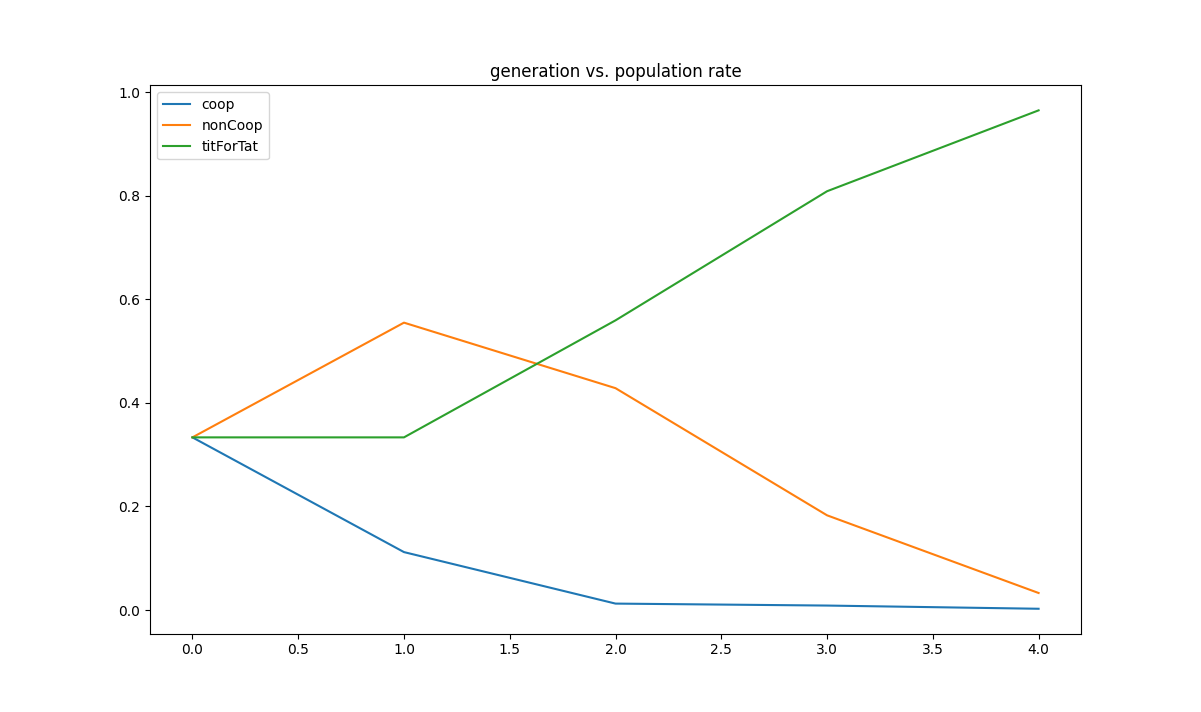
\includegraphics[width = 0.75\textwidth]{images/performance_strategies_repeated}
        \centering
        \caption{The figures shows the performance of the three strategies 'cooperation', 'no cooperation', and 'tit for tat'.}
    \end{figure}
\end{example}

        \newpage

    \section{Appendix}
        \subsection{Linear programs}

    Let $A\in\reals^{n\times k}$, $b\in\reals^{n}, c\in\reals^{k}$. A linear program is a constrained optimisation problem of the following form
    \footnote{This form of a linear program is called standard form. }
    \begin{align*}
        (LP)
        \begin{cases}
            \min_{x\in\reals^{k}}cx^{T} ~\text{ subject to}\\
            ~~~~ Ax^{T}\leq b^{T}\\
            ~~~~ x\geq \mathbf{0}
        \end{cases}
    \end{align*}
    where $\mathbf{0}$ denotes the vector containing only zeros and all the inequality relations are to be understood componentwise. The polyhedron
    \begin{equation*}
        \mathcal{F} = \{x\in\reals^{k} : x\geq\mathbf{0}, Ax^{T}\leq b^{T}\}
    \end{equation*}
    is called the feasible set of $(LP)$. It can be shown that any solution to $(LP)$, if it exists, can be found among the vertices of $\mathcal{F}$. For small
    problems this result leads in a feasible algorithm to solve $(LP)$:
    \begin{enumerate}
        \item Find all the vertices of $\mathcal{F}$
        \item Evaluate the objective function $f(x) = cx^{T}$ among the vertices
        \item The solution of $(LP)$ is the vertex minimising $f$.
    \end{enumerate}
    For large problems however the numerical costs of this approach are too large. This is 
    why the simplex method comes into play, which tries to reduce the number of vertices which have to be visited.

    \begin{example}
        Consider the optimisation problem
        \begin{align*}
            \begin{cases}
                \min -x_{1} - 3x_{2} ~\text{ subject to}\\
                ~~~~ 2x_{1} + 3x_{2}\leq 6\\
                ~~~~ x_{1} - x_{2}\geq -1\\
                ~~~~ x_{1}, x_{2} \geq 0
            \end{cases}                        
        \end{align*}
        In order to write this problem as linear program let us first note that
        \begin{equation*}
            x_{1} - x_{2}\geq -1 \iff -x_{1} + x_{2}\leq 1.
        \end{equation*}
        Definining the matrix $A$, and the vectors $b, c$ via
        \begin{align*}
            A = 
            \begin{bmatrix}
                2 & 3\\
                -1 & 1\\
            \end{bmatrix}, 
            ~b = (6, 1), ~c = (-1, -3)
        \end{align*}
        we infer that the given problem can be rewritten as linear program. The feasible set is depicted in the upfollowing figure. \newline
        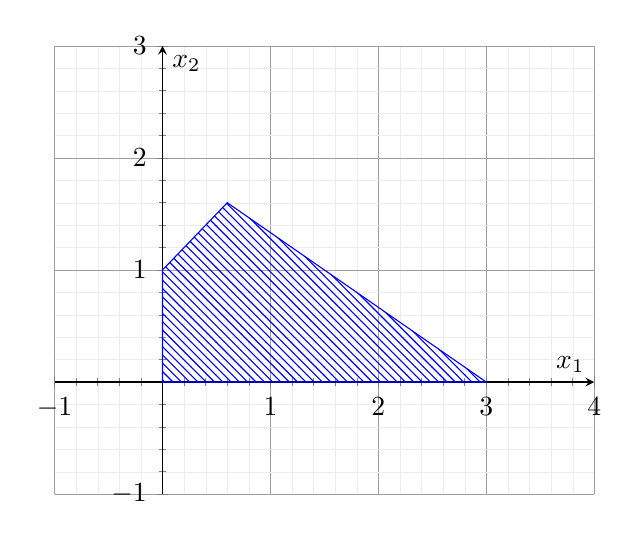
\begin{tikzpicture}
            \begin{axis}
            [
                xmin = -1, xmax = 4,
                ymin = -1, ymax = 3,
                xlabel = {$x_{1}$},
                ylabel = {$x_{2}$},
                grid = both,
                grid style = {line width = .1pt, draw = darkgray!10},
                major grid style = {line width = .2pt, draw = darkgray!50},
                axis lines = middle,
                minor tick num = 4,
                % enlargelimits = {abs = 0.5},
                samples = 100,
                % domain = -20:20,
            ]
            \filldraw[blue, pattern = north west lines, pattern color = blue] (0, 0) -- (0, 1) -- (0.6, 1.6) -- (3, 0) -- cycle;
            \end{axis}
        \end{tikzpicture}
        \newline
        As the figure shows, the feasible set has four vertices, namely $(0, 0), (1, 0), (3 / 5, 8 / 5), (3, 0)$. Moreover we infer that the 
        feasible set is compact. Thus thelinear problem has a solution, which can be found among the vertices of its feasible set. By comparing the 
        values of the objective function $f(x_{1}, x_{2}) = -x_{1} - 3x_{2}$ at the vertices we find that $(3 / 5, 8 / 5)$ solvers the problem.
    \end{example}

        \newpage

    \bibliographystyle{plain}
    \bibliography{myBib}

\end{document}